\documentclass{article}
\author{Daniel Monjas Miguélez}

\title{Topología II: Conceptos Básicos}

\usepackage[spanish]{babel}
\usepackage[utf8]{inputenc}
\usepackage{hyperref}
\usepackage{amsmath}
\usepackage{amssymb}
\usepackage{ textcomp }
\usepackage{ graphicx }
\graphicspath{ {images/} }

\begin{document}
\maketitle
\newpage
\tableofcontents
\newpage

\section{Grupo Fundamental}
\subsection{Homotopías}
\textbf{Definición:} Sea $X$ un espacio topológico. Un lazo en $X$ con base un punto del espacio, $x\in X$ es un arco $\alpha:[0,1]\rightarrow X$ continuo con $\alpha(0)=\alpha(1)=x$. Se denota $\Omega_{x}(X)$ al conjunto de todos los lazos en $X$ con base $x$. \\

Sean $\alpha,\:\beta\in \Omega_{x}(X)$, se define el producto de lazo como
\begin{gather*}
\alpha*\beta:[0,1]\rightarrow X \\
(\alpha*\beta)(t)=\left\lbrace \begin{array}{c}
\alpha(2t)\quad si\:0\leq t\leq \frac{1}{2} \\
\beta(2t-1)\quad si\:\frac{1}{2}\leq t\leq 1
\end{array} \right.
\end{gather*}

\textbf{Definción:} Sean $\alpha,\:\beta\in \Omega_x(X)$, se dicen que son homotópicos, y se denota por $\alpha\simeq \beta$, si existe una aplicación:
\begin{equation*}
H:[0,1]\times[0,1]\rightarrow X\quad continua\:y:
\end{equation*}

\begin{itemize}
\item $H(t,0)=\alpha(t)\quad \forall t\in [0,1]$, es decir, $H(*,0)=\alpha$.

\item $H(t,1)=\beta(t)\quad \forall t\in [0,1]$, es decir, $H(*,1)=\beta$.

\item $H(0,s)=H(1,s)=x\quad \forall s\in [0,1]$, es decir, $H(0,*)=H(1,*)=\varepsilon_x$
\end{itemize}

Se dice que $H$ es un homotopía de $\alpha$ a $\beta$, y se escribe:
\begin{equation*}
H:\alpha\simeq \beta
\end{equation*}

\textbf{Propiedades de las homotopías:}
\begin{enumerate}
\item Si $\alpha\in \Omega_x(X)$, entonces $\alpha\simeq \alpha$ con $H:[0,1]\times [0,1]\rightarrow X$ tal que $H(t,s)=~\alpha(t)$.

\item Si $h:[0,1]\rightarrow [0,1]$ es un homomorfismo con $h(0)=0$ y $h(1)=1$ entonces $\alpha\simeq \alpha\circ h$ donde $\alpha \circ h$ es un reparametrización de $\alpha$ preservando orientación.

\item Sea $\alpha,\beta \in \Omega_x(X)$. Si $\alpha\simeq \beta$ entonces $\beta \simeq \alpha$.

\item Sean $\alpha,\:\beta\in \Omega_x(X)$. Si $\alpha\simeq \beta$ y $\beta\simeq \gamma$ entonces $\alpha\simeq \gamma$.
\end{enumerate}

\textbf{Proposición:} Sean $X$ un espacio topológicos y puntos $p,q,r\in X$. Sean $\alpha,\alpha'\in \Omega_{p,q}(X)$ y $\beta,\beta'\in \Omega_{q,r}(X)$ arcos tales que $\alpha\simeq \alpha'$ y $\beta\simeq \beta'$. Entonces $\alpha*\beta\simeq \alpha'*\beta'$.

\textbf{Proposición:} Sean $X$ un espacio topológico y puntos $p,q,r,s\in X$. Sean $\alpha \in \Omega_{p,q}(X)$, $\beta\in \Omega_{q,r}(X)$ y $\gamma\in \Omega_{r,s}(X)$. Las siguientes propiedades son ciertas:

\begin{itemize}
\item $\alpha*(\beta*\gamma)=(\alpha*\beta)*\gamma)$

\item $(\alpha*\varepsilon_p=\varepsilon_p*\alpha=\alpha$

\item $	\alpha*\overline{\alpha} = \varepsilon_p$
\end{itemize}

\subsection{Grupo Fundamental}
\textbf{Teorema:} Sea $X$ un espacio topológico y $p\in X$ un punto arbitrario. La ley de composición interna
\begin{equation*}
*:\Pi_1(X,p)\times\Pi_1(X,p)\rightarrow\Pi_1(X,p)\qquad [\alpha]*[\beta]=[\alpha*\beta]
\end{equation*}

está bien definida y dota al conjunto $\Pi_1(X,p)$ de estructura de grupo algebraico.

El grupo $(\Pi_1(X,p),*)$ es conocido como \textbf{Grupo Fundamental o de Poincaré} del espacio en el punto $p$. Recalcar que $\Pi_1(X,p)=\Omega_p(X)/\simeq$.\\

\textbf{Proposición:} Sea $(X,\tau)$ un espacio arcoconexo, $x,y\in X$. Entonces los grupos $\Pi_1(X,x)$ y $\Pi_1(X,y)$ son isomorfos.\\

\textbf{Observación:} Sea $\gamma$ un arco que une los puntos $x_1,x_2\in X$ entonces 
\begin{equation*}
\phi:\Pi_1(X,x_1)\rightarrow \Pi_1(X,x_2),\qquad \phi([\alpha])=[\gamma^{-1}][\alpha][\gamma]
\end{equation*}

es un isomorfismo de grupos. \\

\textbf{Corolario:} El grupo fundamental $\Pi_1(X,p)$ está unívocamente determinado salvo isomorfismos por la arcocomponente $C_p$ del punto $p$. En particular, si $X$ es arcoconexo entonces la clase de isomorfía de $\Pi_1(X,p)$ no depende del punto $p\in X$. En este caso la notación es $\Pi_1(X)$. \\

\textbf{Proposición:} Sean $X$ e $Y$ espacios topológicos y $\varphi:X\rightarrow Y$ una aplicación continua. Consideremos $\alpha,\beta\in \Omega_{p,q}(X)$ y los correspondientes $\varphi\circ\alpha,\varphi\circ\beta\in \Omega_{\varphi(p),\varphi(q)}(Y)$. Se tiene que

\begin{equation*}
\alpha\simeq \beta \Rightarrow \varphi\circ \alpha \simeq \varphi\circ\beta
\end{equation*}

En particular:
\begin{itemize}
\item La aplicación $\varphi_*:\Pi_1(X,p)\rightarrow \Pi_1(Y,\varphi(p)),\quad\varphi_*([\alpha])=[\varphi\circ\alpha]$ está bien definida y es un homomorfismo de grupos.

\item Si $\psi:Y\rightarrow Z$ es otra aplicación continua y consideramos los homomorfismos de grupos 
\begin{gather*}
\psi_*:\Pi_1(X,\varphi(p))\rightarrow \Pi_1(Y,\psi(\varphi(p)))\\(\psi\circ\varphi)_*~:~\Pi_1(X,p)~\rightarrow~\Pi_1(Z,\psi(\varphi(p)))
\end{gather*}
entonces se tiene que $(\psi\circ\varphi)_*=\psi_*\circ\varphi_*$
\end{itemize}

\textbf{Corolario (Invarianza topológica del Grupo Fundamental):} Si $\varphi:X\rightarrow Y$ es un homeomorfismo de espacios topológicos entonces $\phi_*:\Pi_1(X,p)\rightarrow \Pi_1(Y,f(p))$ es un isomorfismo de grupos.\\

\textbf{Proposición:} El grupo fundamental de un subconjunto estrellado de $\mathbb{R}^n$ es trivial. En particular, todo subconjunto convexo de $\mathbb{R}^n$ tiene grupo fundamental trivial.

Además, se tiene que 
\begin{equation*}
\Pi_1(X\times Y,(p,q))\cong\Pi_1(X,p)\times \Pi_1(Y,q)
\end{equation*}

\textbf{Observación importante:} El grupo fundamental de $S^n$ es $\mathbb{Z}$. El grupo fundamental de un conjunto $X$ estrellado es $\Pi_1(X,x)=\{[\epsilon_x]\}$.

El grupo fundamental del toro $T=S^1\times S^1$ es $\mathbb{Z}\times \mathbb{Z} = \mathbb{Z}^2$.

El grupo fundamental del cilindro $S^n\times \mathbb{R}$ es $\mathbb{Z}\times\{1\}\cong \mathbb{Z}$. El grupo fundamental de $X$ estrellado es $\Pi_1(S^1,1)=(\{[\alpha_n]:n\in \mathbb{N},*\})$.\\

\textbf{Definición:} Un grupo topológico es un par $(G,.)$ donde:
\begin{itemize}
\item $G$ es un espacio topológico.

\item $.:G\times G\rightarrow G$ es una ley de composición interna en $G$ que le dota de estructura algebraica.

\item La aplicación $G\times G\rightarrow G\quad (a,b)\rightarrow a. b^{-1}$ es continua, o equivalentemente: $.:G\times G\quad (a,b)\mapsto a.b$ y $(~)^{-1}:G\rightarrow G\quad a\rightarrow a^{-1}$ son continuas.
\end{itemize}

\textbf{Propiedad del levantamiento de arco:} Sea $\alpha:[0,1]\rightarrow S^1$ un arco con $\alpha(0)=1$. Entonces existe un único arco $\tilde{\alpha}:[0,1]\rightarrow \mathbb{R}$ tal que $\rho \circ \tilde{\alpha}=\alpha$ y $\tilde{\alpha}(0)=0$, donde $\rho:\mathbb{R}\rightarrow S^1$, $\rho(t)=e^{2\pi it}=(cos(2\pi t), sen(2\pi t))$. \\

\textbf{Propiedad del levantamiento de homotopías:} Sea $\alpha,\beta:[0,1]\rightarrow S^1$ un arco con $\alpha(0)=\beta(0)=1$ y $\alpha(1)=\beta(1)$. Supongamos que existe una homotopía $H$ de $\alpha$ en $\beta$. Entonces:
\begin{itemize}
\item Los arcos $\tilde{\alpha}$ y $\tilde{\beta}$ tienen los mismos extremos.

\item La aplicación $\tilde{H}$ es una homotopía (con extremos fijos) de $\tilde{\alpha}$ en $\tilde{\beta}$, donde $\tilde{H}:[0,1]^2\rightarrow \mathbb{R}$ es continua y tal que $\rho \circ \tilde{H}=H$ y $\tilde{H}(0,0)=0$.
\end{itemize}

\textbf{Definición:} Si $\alpha \equiv (\alpha_1,\alpha_2):[0,1]\rightarrow S^1\subset \mathbb{R}^2$ es un arco de clase $C^1$ con $\alpha(0)=(1,0)$, entonces su levantamiento vía $\rho$ a $\mathbb{R}$ dado por:
\begin{equation*}
\tilde{\alpha}(t)=\frac{1}{2\pi}\int_0^t (\alpha_1(s)\alpha_2'(s)-\alpha_1'(s)\alpha_2(s))ds
\end{equation*}

De forma explícita, y para cada $n\in \mathbb{Z}$, el lazo $\alpha_n:[0,1]\rightarrow S^1\subset \mathbb{C}$, $\alpha_n(t)=e^{2n\pi it}$ se levanta con condición inicial $\tilde{\alpha}_n(0)=0$ al arco $\tilde{\alpha}_n:[0,1]\rightarrow\mathbb{R}$, $\tilde{\alpha}_n(t)=nt$.\\

\textbf{Definición:} Dado un lazo $\alpha:[0,1]\rightarrow S^1$ con base el punto $1\in S^1$, definimos el grado de $\alpha$ como:
\begin{equation*}
deg(\alpha)=\tilde{\alpha}(1)\in \mathbb{Z}
\end{equation*}

donde $\tilde{\alpha}:[0,1]\rightarrow\mathbb{R}$ represental el levantamiento de $\alpha$ con condición inicial $\tilde{\alpha}(0)=0$.\\

\textbf{Proposición:} Dados $\alpha,\beta:[0,1]\rightarrow S^1$ dos lazos con base $1\in S^1$, se tiene que 
\begin{equation*}
\alpha\simeq \beta\Leftrightarrow deg(\alpha)=deg(\beta)
\end{equation*}

\textbf{Teorema:} La aplicación 
\begin{gather*}
deg:(\Pi_1(S^1,1),*)\rightarrow (\mathbb{Z},+),\\
deg([\alpha])=deg(\alpha)
\end{gather*}

\textbf{Proposición:} Si $\overline{D}$ denota el disco unidad cerrado $\overline{D}=\{(x,y)\in \mathbb{R}^2:x^2+y^2\leq 1\}$, no existe ninguna aplicación continua $f:\overline{D}\rightarrow S^1$ tal que $f_{|_{S^1}}=Id_{S^1}$. \\

\textbf{Teorema (Punto fijo de Brower):} Sea $f:\overline{D}\rightarrow \overline{D}$ una aplicación continua. Entonces existe $p_0\in \overline{D}$ tal que $f(p_0)=p_0$. \\

\subsection{Retracciones y Retractos de Deformación}
\textbf{Teorema Fundamental del Álgebra:} Sea $P:\mathbb{C}\rightarrow C$ una función polinómica de la forma
\begin{equation*}
P(z)=a_0+\ldots+a_{n-1}z^{n-1}+z^n\qquad n\geq 1
\end{equation*}
Entonces existe $z_0\in \mathbb{C}$ tal que $P(z_0)=0$.\\

\textbf{Definición:} Sea $X$ un espacio topológico y $A\subset X$ un subespacio topológico. Una retracción o retracto de $X$ en $A$ es una aplicación continua $r:X\rightarrow A$ satisfaciendo $r_{|_A}=Id_A$, o equivalentemente, $r\circ i=Id_A$ donde $i:A\rightarrow X$ es la aplicación inclusión, $i(x)=x$. En este caso se dice que $A$ es un retractor de $X$. \\

\textbf{Proposición:} Sea $r:X\rightarrow A$ es una retracción, $i:A\rightarrow X$ la aplicación inclusión y $a\in A$, entonces:
\begin{itemize}
\item $r_*:\Pi_1(X,a)\rightarrow\Pi_1(A,a)$ es un epimorfismo.

\item $i_*:\Pi_1(A,a)\rightarrow\Pi_1(X,a)$ es un monomorfismo.
\end{itemize}

\textbf{Definición (Retracto de deformación):} Dado un espacio topológico $X$ y un subespacio $A\subset X$, se dice que $A$ es un retracto de deformación de $X$ si existen una retracción $r:X\rightarrow A$ y una aplicación continua $H:X\times[0,1]\rightarrow X$ satisfaciendo:
\begin{equation*}
H(x,0)=x\quad \forall x\in X\qquad H(x,1)=r(x)\quad \forall x\in X
\end{equation*}

Si adicionalmente $H(a,s)=a\quad \forall(a,s)\in A\times [0,1]$, entonces se dice que $A$ es un retracto fuerte de deformación de $X$. A las aplicaciones $H$ y $r$ se les llamará deformación y retracción asociadas al retracto (fuerte) de deformación $A$ de $X$, respectivamente.\\

\textbf{Proposición:} Si $A$ es un retracto de deformación de $X$, $\{C_\alpha:\alpha\in \Lambda\}$ son las arcocomponentes de $A$ y $\hat{C}_\alpha$ es la arcocomponente de $X$ conteniendo a $C_\alpha$ para cada $\alpha\in \Lambda$, entonces:
\begin{enumerate}
\item $r(\hat{C}_\alpha)=C_\alpha \quad \forall\alpha\in\Lambda$ y por tanto, $\hat{C}_\alpha\neq \hat{C}_\beta,\:\alpha\neq \beta$.

\item $\{C_\alpha:\alpha\in\Lambda\}$ son las arcocomponentes de $X$.

\item Si $H:X\times [0,1]\rightarrow X$ y $r:X\rightarrow A$ son una deformación y retracción asociadas al retracto de deformación $A$ de $X$, entonces $H_{|\hat{C}_\alpha\times[0,1]}:\hat{C}_\alpha\times[0,1]\rightarrow \hat{C}_\alpha$ y $r_{|\hat{C}_\alpha}:\hat{C}_\alpha\rightarrow C_\alpha$ son una deformación y retracción asociadas al retracto de deformación $C_\alpha$ de $\hat{C}_\alpha$.
\end{enumerate}

\textbf{Proposición:} Sea $F:X\rightarrow A$ un homeomorfismo. Si $A$ es un retracto (fuerte) de deformación de $Y$ entonces $F^{-1}(A)$ es un retracto (fuerte) de deformación de $X$. \\

\textbf{Teorema:} Sea $X$ un espacio topológico y sea $A\subset X$ un retracto fuerte de deformación con $r:X\rightarrow A$ una retracción asociada. Entonces dado $a\in A$ se tiene que:
\begin{equation*}
r_*:\Pi_1(X,a)\rightarrow \Pi_1(A,a)\qquad i_*:\Pi_1(A,a)\rightarrow \Pi_1(X,a)
\end{equation*}

son isomorfismos, uno inverso del otro.\\

\textbf{Definición:} Un espacio topológico $X$ se dice contráctil si admite como retracto de deformación a un punto $\{p_0\}\subset X$. En caso de que $\{p_0\}$ sea retracto fuerte de deformación de $X$ diremos que el espacio es fuertemente contráctil.\\

\textbf{Definición:} Un espacio topológico $X$ se dice simplemente conexo si es arcoconexo y $\Pi_1(X,p)=\{[\epsilon_p]\}$ para algún $p\in X$ (luego para todo $p\in X$).\\

\textbf{Corolario:} Todo espacio fuertemente contráctil es simplemente conexo.\\

\textbf{Consecuencias:} 
\begin{enumerate}
\item Todo subconjunto estrellado de $\mathbb{R}^n$ es simplemente conexo. Esto se aplica a subconjuntos $A\subset \mathbb{R}^n$ convexos.

\item Si $p\in S^n$ entonces $\Pi_1(\mathbb{R}^{n+1}-\{0\},p)$ es isomorfo a $\Pi_1(S^n,p)$.

\item Si $p\in S^1$ entonces $\Pi_1(S^1\times \mathbb{R},(p,0))$ es isomorfo a $\Pi_1(S^1,p)\cong \mathbb{Z}$.

\item Si $p\in S^1\times \mathbb{R}$ entonces $\Pi_1(\mathbb{R}^3-\{x=y=0\},p)$ es isomorfo a $\Pi_1(S^1\times \mathbb{R},p)\cong \mathbb{Z}$.

\item El grupo fundamental de la cinta de Möbius es isomorfo a $\mathbb{Z}$.
\end{enumerate} 

\textbf{Definición:} Sea $(X,\tau)$ espacio topológico.
\begin{enumerate}
\item Se dice que el espacio satisface el primer axioma de numerabilidad (o ANI) si todo punto tiene una base numerable de entronos.

\item Se dice que el espacio satisface el segundo axioma de numerabilidad (o ANII) si la topología tiene una base numerable.
\end{enumerate}

\textbf{Teorema:} Sea $X$ un espacio topológico conexo y localmente arcoconexo. Supongamos que la topología admite una base $\beta$ satisfaciendo:
\begin{enumerate}
\item $\beta$ es numerable (luego $X$ es II-Axioma de Numerabilidad).

\item $B$ es simplemente conexo $\forall B\in \beta$.
\end{enumerate}
Entonces $\Pi_1(X,x)$ es numerable $\forall x\in X$. \\

\subsection{Homotopías de aplicaciones}
\textbf{Definición (Homotopía de aplicaciones):} Dados dso espacios topológicos $X$ e $Y$, dos aplicaciones continuas $\varphi_1,\varphi_2:X\rightarrow Y$, se dicen homotópicas, y se escribe $\varphi_1\simeq \varphi_2$, si existe una aplicación $H:X\times [0,1]\rightarrow Y$ verificando:
\begin{equation*}
H(x,0)=\varphi_1(x)\forall x\in X\qquad H(x,1)=\varphi_2(x)\forall x\in X
\end{equation*}

Si $A\subset X$, las aplicaciones continuas $\varphi_1,\varphi_2:X\rightarrow Y$ se dirán homotópicas relativas a $A$, $\varphi_1\simeq_A\varphi_2$ si existe $H:X\times [0,1]\rightarrow Y$ verificando:
\begin{gather*}
H(x,0)=\varphi_1(x)\quad \forall x\in X\qquad H(x,1)=\varphi_2(x)\quad \forall x\in X\\
H(a,s)=\varphi_1(a)=\varphi_2(a)\quad \forall(a,s)\in A\times [0,1]
\end{gather*}
Si $A\subset X$ es un retracto de deformación vía $H$ con la retracción asociada $r$, entonces $Id_X\simeq r$. Si $A$ es un retracto fuerte de deformación de $X$ se tiene que $Id_X\simeq_A r$.\\

\textbf{Teorema:} Sean $X$ e $Y$ espacios topológicos y dos aplicaciones continuas $\varphi_1,\varphi_2:X\rightarrow Y$. Supongamos que $\varphi_1\simeq\varphi_2$ vía $H:X\times [0,1]\rightarrow Y$, fijemos $x_0\in X$ y sea $\gamma:[0,1]\rightarrow Y$ el arco uniendo $\varphi_1(x_0)$ y $\varphi_2(x_0)$ definido por $\gamma(s)=H(x_0,s)$. \\

Dados los homomorfismos de grupos
\begin{equation*}
(\varphi_1)_*:\Pi_1(X,x_0)\rightarrow \Pi_1(Y,\varphi_1(x_0))\qquad (\varphi_2)_*:\Pi_1(X,x_0)\rightarrow \Pi_1(Y,\varphi_2(x_0))
\end{equation*}
Y el isomorfismo $U_\gamma:\Pi_1(Y,\varphi_1(x_0))\rightarrow \Pi_1(Y,\varphi_2(x_0))$, se tiene que $U_\gamma\circ (\varphi_1)_*=(\varphi_2)_*$. En particular, los homomorfismos $(\varphi_1)_*$ y $(\varphi_2)_*$ son iguales salvo isomorfismo. \\

\textbf{Corolario:} Sean $\varphi_1,\varphi_2:X\rightarrow Y$ aplicaciones continuas y $x_0\in X$. Supongamos que $\varphi_1\simeq_{\{x_0\}}\varphi_2$ y sea $y_0=\varphi_1(x_0)=\varphi_2(x_0)$. Entonces $(\varphi_1)_*=(\varphi_2)_*:\Pi_1(X,x_0)\rightarrow \Pi_1(Y,y_0)$.\\

\textbf{Definición:} Sean $X$ e $Y$ espacios topológicos. Una aplicación continua $f:X\rightarrow Y$ se dirá una equivalencia homotópica si existe $g:X\rightarrow Y$ tal que $g\circ f=Id_X$ y $f\circ g=Id_Y$. En ese caso se dirá que $f$ y $g$ son inversas homotópicas. \\

Dos espacios $X$ e $Y$ se dicen del mismo tipo de homotopía si existe una equivalencia homotópica entre ellos. \\

\textbf{Nota:} Todo homeomorfismo es una equivalencia homotópica pero el recíproco no es cierto. La equivalencia homotópica es suficiente para garantizar isomorfismo entre grupos fundamentales. \\

\textbf{Teorema:} Sean $X$ e $Y$ espacios topológicos y $f:X\rightarrow Y$ una equivalencia homotópica con inversa homotópica $g:X\rightarrow Y$. Fijemos $x_0\in X$. Entonces $f_*:\Pi_1(X,x_0)\rightarrow \Pi_1(Y,f(x_0))$ es un isomorfismo de grupos. \\

\textbf{Corolario:} Sea $A\subset X$ es un retracto de deformación de $X$ con la retracción asociada $r:X\rightarrow A$ e $i:A\rightarrow X$ la aplicación inclusión. Entonces para cada $a\in A$ las aplicaciones 
\begin{equation*}
r_*:\Pi_1(X,a)\rightarrow \Pi_1(A,a)\qquad i_*:\Pi_1(A,a)\rightarrow \Pi_1(X,a)
\end{equation*}
son isomorfismos de grupos. En particular, todo espacio topológico contráctil es simplemente conexo. \\

\textbf{Proposición:} Sea $X$ un espacio topológico, y sean $U,V\subset X$ subconjuntos satisfaciendo:
\begin{enumerate}
\item $U$ y $V$ son abiertos simplemente conexos (con la topología inducida).

\item $U\cap V$ es arcoconexo y no vacío.

\item $U\cup V=X$
\end{enumerate}
Entonces $X$ es simplemente conexo.\\

\textbf{Corolario:} La esfera $S^n$ es simplemente conexa para todo $n\geq 2$. \\

\textbf{Teorema de Invarianza de la Dimensión:} Si $\Omega_2\subset \mathbb{R}^2$ y $\Omega_n\subset \mathbb{R}^n$ con $n\neq 2$ son abiertos conexos, entonces $\Omega_2$ no es homeomorfo a $\Omega_n$.\\

\textbf{Lema:} No existe ninguna aplicación $F:S^2\rightarrow S^1$ continua e impar. \\

\textbf{Teorema (Borsuk-Ulam):} Si $f:S^2\rightarrow \mathbb{R}^2$ es continua, entonces existes $x_0\in S^2$ tal que $f(x_0)=f(-x_0)$. \\

\textbf{Corolario:} Si identificamos $S^2$ con la superficie de la tierra y $f,g:S^2\rightarrow \mathbb{R}$ son dos magnitudes físicas que se distribuyen de forma continua sobre dicha superficie (por ejemplo, la presión y la temperatura), existen puntos antípodas $p_0,-p_0\in S^2$ tales que $(f,g)(p_0)=(f,g)(-p_0)$.\\

\textbf{Corolario:} Si $S^2$ es la unión de tres subconjuntos cerrados $A_1,A_2$ y $A_3$, entonces alguno de ellos contiene dos puntos antípodas.\\

\textbf{Corolario (Teorema de las tortitas):} Dados dos compactos $A_1,A_2\subset \mathbb{R}^2$, existe una recta combinatoria de $\mathbb{R}^2$ que los subdivide a ambos en trozos de igual área. \\

\textbf{Corolario (Teorema del bocadillo de jamón):} Dados tres compactos $A_1,A_2,A_3\in \mathbb{R}^3$, es posible encontrar un plano combinatorio de $\mathbb{R}^3$ que los subdivida a los tres en trozos de igual volumen. \\

\subsection{Teorema de Seifert-Van Kampen}
\textbf{Teorema de Seifert-Van Kampen:} Sea $X$ un espacio topológico y sean $U,V\subset X$ subconjuntos satisfaciendo:
\begin{enumerate}
\item $U,V$ y $U\cap V$ son abiertos arcoconexos.

\item $U\cap V\neq \emptyset$ y $U\cup V=X$
\end{enumerate}

$i_*:\Pi_1(U\cap V,x_0)\rightarrow \Pi_1(U,x_0)$ y $j_*:\Pi_1(U\cap V,x_0)\rightarrow \Pi_1(V,x_0)$ los correspondientes homomorfismos inducidos. Entonces
\begin{equation*}
\Pi_1(X,x_0)\cong \Pi_1(U,x_0)*_{\Pi_1(U\cap V,x_0)}\Pi_1(V,x_0)
\end{equation*}
donde el producto amalgamado es el relativo a los homomorfismos $i_*$ y $j_*$.\\

\textbf{Corolario:} Bajo las mismas hipótesis del Teorema de Seifert-Van Kampen, si $U\cap V$ es simplemente conexo entonces $\Pi_1(X,x_0)\cong \Pi_1(U,x_0)*\Pi_1(V,x_0)$. \\

\textbf{Corolario:} Bajos las mismas hipótesis del Teorema de Seifert-Van Kampen, si $V$ es simplemente conexo entonces 
\begin{equation*}
\Pi_1(X,x_0)\cong \Pi_1(U,x_0)/N(i_*(Pi_1(U\cap V,x_0)))
\end{equation*}

\textbf{Definición:} Si $A$ es un subconjunto de $G$:
\begin{itemize}
\item $N(A):=\left\lbrace \prod_{j=1}^k g_j^{-1}\cdot a_j^{n_j}\cdot g_j:(a_j,g_j,n_j)\in A\times G\times \mathbb{Z},\quad j=1,\ldots,k,\quad k\in \mathbb{N}\right\rbrace$ es el menor subgrupo normal de $G$ conteniendo a $A$, también llamado el subgrupo normal de $G$ generado por $A$. Es fácil comprobar que $N(A)$ coincide con la intersección de todos los subgrupos normales de $G$ que contienen a $A$.

\item Si $H\leq G$, $N_0(H):=\{g\in G:g^{-1}\cdot H\cdot g=H\}$ es el mayor subgrupo de $G$ que contiene a $H$ como subgrupo normal, también llamado el normalizador de $H$ en $G$. Es claro que $H\unlhd N_0(H)\leq G$ y $N_0(H)=G$ si y solo si $H\unlhd G$.
\end{itemize}

\textbf{Corolario:} Si $X$ es un n-ciclo entonces $\Pi_1(X,x_0)$ es isomorfo al grupo libre $F(a_1,\ldots,a_n)$. \\

\textbf{Definición:} Sea el semiplano $\Pi_1=\{(x_1,x_2,x_3)\subset \mathbb{R}^3:x_1=0,x_2\geq 0\}$ y sus girados respecto del eje $x_3$:
\begin{equation*}
\Pi_j=\{\left(e^{2\pi(j-1)i/k}z,x_3\right):(z,x_3)\in \Pi_1\subset \mathbb{C}\times \mathbb{R}\equiv \mathbb{R}^3\}\quad j=1,\ldots,k
\end{equation*}
Por definición, el espacio libre de $k$ hojas es:
\begin{equation*}
L_k=\bigcup_{j=1}^k\Pi_j\qquad k\in\mathbb{N}
\end{equation*}

\textbf{Proposición:} Los espacios $L_k$ y $L_s$ no son homeomorfos, $k,s\in \mathbb{N}$, $k\neq s$.\\

\textbf{Corolario:} Si $O\subset \mathbb{R}^3$ es un abierto conteniendo al origen, entonces $O\cap L_k$ no puede ser homeomorfo a un abierto de $\mathbb{R}^2$ para todo $k\neq 2$.

\section{Espacios recubridores}
\subsection{Definiciones y nociones básicas}
\textbf{Definición:} Sea $X$ un espacio topológico. Un (espacio) recubridor de $X$ es un par $(\tilde{X},\pi)$, donde:
\begin{enumerate}
\item $\tilde{X}$ es un espacio topológico.

\item $\pi:\tilde{X}\rightarrow X$ es una aplicación continua y sobreyectiva.

\item Todo punto $p\in X$ admite un entorno abierto y arcoconexo $U$ en $X$ tal que $\pi_{|U}:\tilde{U}\rightarrow U$ es un homeomorfismo para toda arcocomponente $\tilde{U}$ de $\pi^{-1}(U)$
\end{enumerate}

\begin{figure}[h]
\centering
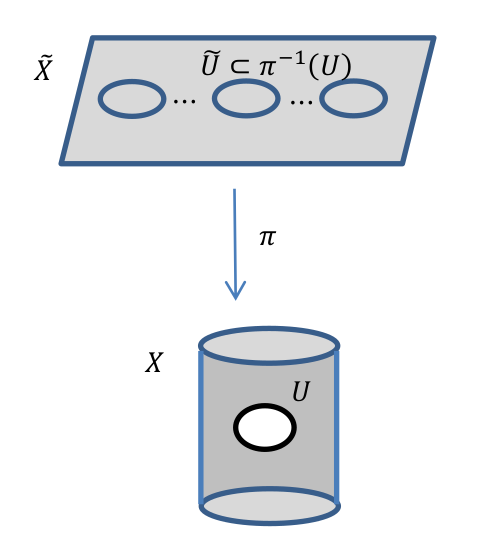
\includegraphics[scale=1,width=7cm, height=8cm]{recubridor.png}
\end{figure}

Al abierto $U$ se le llamará entorno fundamental o distinguido para el recubridor $(\tilde{X},\pi)$. A al aplicación $\pi$ se la llamará aplicación recubridora, y al espacio $X$ base del recubridor $(\tilde{X},\pi)$, y a $\tilde{X}$ el espacio recubridor. \\

Dado $p\in X$, al conjunto $\pi^{-1}(p)\subset \tilde{X}$ se le llama fibra del punto $p$ para el recubridor $(\tilde{X},\pi)$. Un recubridor se dirá finito (y la aplicación recubridora finita) cuando la fibra $\pi^{-1}(p)$ sea finita para todo $p\in X$. \\

La familia $\mathcal{U}=\{U\subset X:U\:es\:entorno\:distinguido\:para\:(\tilde{X},\pi)\}$ es una base de la topología de $X$. Cada arcocomponente $\tilde{U}$ de $\pi^{-1}(U)$ es un subconjunto abierto de $\tilde{X}$. Además, la aplicación $\pi$ es abierta, y el conjunto de arcocomponente de $\pi^{-1}(U)$ está en correspondencia uno a uno con la fibra de $p$.\\

\textbf{Ejemplos imortantes de aplicaciones recubridoras:}
\begin{itemize}
\item La aplicación exponencial $\rho:\mathbb{R}\rightarrow \mathbb{S}^1$, $\rho(t)=e^{2\pi i t}$. Es decir, $\mathbb{R}$ recubre a $S^1$.

\item De la anterior se induce que $\rho\times \rho:\mathbb{R}^2\rightarrow \mathbb{S}^1\times \mathbb{S}^1=\mathbb{T}$. Es decir, $\mathbb{R}^2$ recubre al toro de revolución.

\item Un homeomorfismo $f:X\rightarrow Y$. Es decir, si $X\cong Y$ entonces $X$ recubre a $Y$.

\item La aplicación $\pi_n:\mathbb{S}^1\rightarrow \mathbb{S}^1$, $\pi_n(z):=z^n$.

\item $\pi_1\times \pi_2:Y_1\times Y_2\rightarrow X_1\times X_2$, donde $\pi_j:Y_j\rightarrow X_j$ es recubridora para $j=1,2$.

\item $\rho\times Id_{\mathbb{R}}:\mathbb{R}^2\times \mathbb{S}^1\times \mathbb{R}$
\end{itemize}

\textbf{Proposición:} Si $f:Y\rightarrow X$ es un homeomorfismo local, sobreyectivo y propio entre espacios de Hausodrff localmente compactos, entonces $f$ es una aplicación recubridora finita. \\

\textbf{Corolario:} Supongamos que $X$ e $Y$ son espacios Hausdorff, $Y$ compacto. Todo homeomorfismo local $f:Y\rightarrow X$ es una aplicación recubridora. \\

\textbf{Proposición:} Sean $\pi_1:Y\rightarrow Z$ y $\pi_2:Z\rightarrow X$ aplicaciones recubridoras. Si $\pi_2$ es finita entonces $\pi_2\circ \pi_1: Y\rightarrow X$ es recubridora. \\

\textbf{Definición:} Sea $X$ un espacio topológico, y sea $G\subset Hom(X)$ un subgrupo. Consideremos la acción canónica de $G$ sobre $X$, $\mu:G\times X\rightarrow X$, donde $\mu(g,x)=g(x)$. Es habitual escribir $g.x$ en vez de $\mu(g,x)$ para todo $g\in G$, $x\in X$. La relación binaria en $X$:
\begin{equation*}
x\sim y\Leftrightarrow \exists g\in G: g.x=y2
\end{equation*}

Es de equivalencia. El espacio topológico coeicnete $X/\sim$ se denotará por $X/G$ y será referido como el espacio de órbitas asociado a la acción $\mu$ inducida por $G$. \\

\textbf{Definición:} Sea $X$ espacio topológico, y sea $G\subset Hom(X)$ un subgrupo. El subgrupo $g$ se dirá que actúa de forma propia y discontinua sobre $X$ (y la acción $\mu:G\times X\rightarrow X$ inducida se dirá propia y discontinua) si para todo $x\in X$ existe un entorno abierto $U$ de $x$ en $X$, tal que $(g.U)\cap U=\emptyset$ para todo $g\in G\backslash\{Id_X\}$ (aquí $g.U$ denota el conjunto $g(U)$). Al entrono $U$ se llama entorno distinguido (alrededor de x) para la acción. \\

\textbf{Proposición:} Si $X$ es un espacio topológico Hausdorff y $G$ es un grupo finito de homomorfismos de $X$ sin puntos fijos (esto es, tal que $\phi(x)\neq x$ para todo $e\in X$ y $\phi\in G\backslash\{Id_X\}$), entonces $G$ actúa de forma propia y discontinua sobre $X$.\\

\textbf{Teorema:} Sea $X$ un espacio topológico, y sea $G\subset Hom(X)$ un subgrupo actuando de forma propia y discontinua sobre $X$. Entonces la proyección al espacio de órbitas $\pi:X\rightarrow X/G$ es recubridora.

\subsection{Levantamiento de aplicaciones al recubridor}
\textbf{Proposición:} Sea $(\tilde{X},\pi)$ un recubridor de $X$, sea $Y$ un espacio topológico conexo y sean $f_1,f_2:Y\rightarrow \tilde{X}$ dos aplicaciones continuas satisfaciendo $\pi\circ f_1=\pi\circ f_2$. Si $A=\{y\in Y:f_1(y)=f_2(y)\}\neq\emptyset$ entonces $f_1=f_2$. \\

\textbf{Lema}: Sea $(\tilde{X},\pi)$ un recubridor de $X$, y sean $x_0\in X$ y $\tilde{x}_0\in \pi^{-1}(x_0)$. Dada $H:[0,1]^2\rightarrow X$ continua con $H(0,0)=x_0$, existe una única aplicación $\tilde{H}:[0,1]^2\rightarrow X$ continua tal que $\pi\circ \tilde{H}=H$ y $\tilde{H}(0,0)=\tilde{x}_0$.\\

\textbf{Corolario (Propiedad del levantamiento de arco):} Sea $(\tilde{X},\pi)$ un recubridor de $X$, y sean $x_0\in X$ y $\tilde{x}_0\in \pi^{-1}(x_0)$, y se considera un arco $\alpha:[0,1]\rightarrow X$ con $\alpha(0)=x_0$. Entonces existe un único arco $\tilde{\alpha}:[0,1]\rightarrow \tilde{X}$ tal que $\pi\circ\tilde{\alpha}=\alpha$ y $\tilde{\alpha}(0)=\tilde{x}_0$. A $\tilde{\alpha}$ se le llama levantamiento de $\alpha$ vía $\pi$ con condición inicial $\tilde{\alpha}(0)=\tilde{x}_0$.\\

\textbf{Definición:} Dado un recubridor $(\tilde{X},\pi)$ de $X$, un arco $\alpha:[0,1]\rightarrow X$ con $\alpha(0)=x$ y $\tilde{x}\in \pi^{-1}(x)$, se denota por $\tilde{\alpha}_{\tilde{x}}:[0,1]\rightarrow \tilde{X}$ el único levantamiento de $\alpha$ vía $\pi$ con condición inicial $\tilde{\alpha}(0)=\tilde{x}$.\\

\begin{figure}[h]
\centering
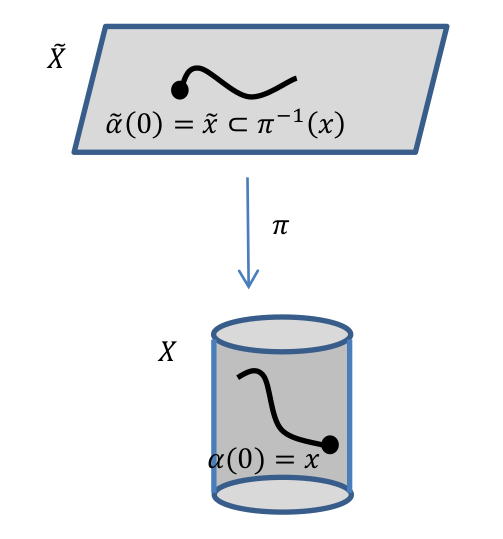
\includegraphics[scale=1,width=6.cm, height=6cm]{levantamientoarco.png}
\end{figure}

\textbf{Corolario:} Sea $(\tilde{X},\pi)$ un recubridor de $X$, y $y\in X$ y un arco $\alpha:[0,1]\rightarrow X$ con $\alpha(0)=x$ y $\alpha(1)=1$. Consideramos la aplicación $n_\alpha:\pi^{-1}(x)\rightarrow \pi^{-1}(y)$ dada por $n_\alpha(\tilde{x})=\tilde{\alpha}_{\tilde{x}}(1)$. Entonces $n_\alpha$ es biyectiva, y en particular $\pi^{-1}(x)$ y $\pi^{-1}(y)$ tienen el mismo cardinal.\\

\textbf{Definición (Número de hojas de un recubridor):} Dado un recubridor $(\tilde{X},\pi)$ de $X$, se llama número de hojas del recubridor al cardinal de $\pi^{-1}(x)$, donde $x$ es un punto aleatorio de $X$.\\

\textbf{Corolario (Propiedad del levantamiento de homotopías):} Sea $(\tilde{X},\pi)$ un recubridor de $X$, y sean $x_0\in X$ y $\tilde{x}_0\in \pi^{-1}(x_0)$, y sean dos arcos $\alpha,\beta:[0,1]\rightarrow X$ con $\alpha(0)=\beta(0)=x_0$ y $\alpha(1)=\beta(1)$. Supongamos que existe una homotopía de $\alpha$ en $\beta$ (con extremos fijos). Entonces, los arcos $\tilde{\alpha}_{\tilde{x}_0}$ y $\tilde{\beta}_{\tilde{x}_0}$ tienen los mismo extremos y la aplicación $\tilde{H}$ es una homotopía de $\tilde{\alpha}$ en $\tilde{\beta}$ (con extremos fijos).\\

\textbf{Teorema de Monodromía:} Sea $(\tilde{X},\pi)$ un recubridor de $X$, y sean $x\in X$ y $\tilde{x}\in \pi^{-1}(x)$, entonces $\pi_*:\Pi_1(\tilde{X},\tilde{x})\rightarrow \Pi_1(X,x)$ es un monomorfismo de grupos.\\

\textbf{Corolario:} Sea $(\tilde{X},\pi)$ es un recubridor de $X$, y sean $x\in X$. Sean $\tilde{x}_1,\tilde{x}_2\in \pi^{-1}(x)$ y $\tilde{\alpha}:[0,1]\rightarrow \tilde{X}$ un arco con $\tilde{\alpha}(0)=\tilde{x}_1$ y $\tilde{\alpha}(1)=\tilde{x}_2$. Entonces
\begin{equation*}
\pi_*\left(\Pi_1(\tilde{X},\tilde{x}_2)\right)=[\alpha]^{-1}*\pi_*\left(\Pi_1(\tilde{X},\tilde{x}_1)\right)
\end{equation*}

donde $\alpha$ es el lazo $\pi\circ \tilde{\alpha}$ (con base $x$). Como consecuencia $\left\lbrace \pi_*(\left(\Pi_1(\tilde{X},\tilde{x})\right):\tilde{x}\in \pi^{-1}(x)\right\rbrace$ es una clase de conjugación de subgrupos en $\Pi_1(X,x)$.\\

\textbf{Definición:} Se denota por $Rec(X)$ el conjunto de todos los recubridores de $X$, esto es:
\begin{equation*}
Rec(X)=\left\lbrace(\tilde{X},\pi):(\tilde{X},\pi)\:es\:un\:recubridor\:de\:X\right\rbrace
\end{equation*}
Fijamos $x\in X$ y sea el conjunto $S_c\left(\Pi_1(X,x)\right)$ de las clases de conjugación de subgrupos de $\Pi_1(X,x)$, se define:
\begin{equation*}
\Delta_x:Rec(X)\rightarrow S_c(\Pi_1(X,x))\qquad \Delta_x(\tilde{X},\pi)=\left\lbrace\pi_*(\Pi_1(\tilde{X},\tilde{x})):\tilde{x}\in \pi^{-1}(x)\right\rbrace
\end{equation*}

\textbf{Teorema:} Sea $\pi:\tilde{X}\rightarrow X$ una aplicación recubridora, sea $f:Y\rightarrow X$ una aplicacón continua y sea $y_0\in Y$, $x_0\in f(y_0)\in X$ y $\tilde{x}_0\in \pi^{-1}(x_0)$. Los siguientes enunciados son equivalentes:
\begin{itemize}
\item Existe $\tilde{f}:Y\rightarrow \tilde{X}$ continua tal que $\pi\circ \tilde{f}=f$ y $\tilde{f}(y_0)=\tilde{x}_0$.

\item $f_*(\Pi_1(Y,y_0))\subset \pi_*(\Pi_1(\tilde{X},\tilde{x}_0))$. 
\end{itemize}

\textbf{Corolario:} Sea $(Y,\pi)$ un recubridor de $X$, sea $A\subset X$ un subespacio topológico arcoconexo y denotemos por $i:A\rightarrow X$ a la aplicación inclusión. Supongamos $i_*(\Pi_1(A,x))\pi(\Pi_1(Y,y))$ para algunos $x\in A$ e $y\in \pi^{-1}(x)$. Entonces $\pi_{|\tilde{A}}:\tilde{A}\rightarrow A$ es un homeomorfismo, donde $\tilde{A}$ es la arcocomponente de $\pi^{-1}(A)$ que contiene a $y$.\\

\textbf{Proposición:} Sea $(G,.)$ un grupo topológico con elemento neutro $e\in G$, sea $\pi:\tilde{G}\rightarrow G$ una aplicación recubridora y elegimos $\tilde{e}\in \pi^{-1}(e)$. Entonces $\tilde{G}$ admite una estructura de grupo topológico con elemento neutro $\tilde{e}$ que conveirte a $\pi$ es un homomorfismo de grupos. \\

\textbf{Corolario:} $X$ tiene como máximo, salvo isomorfismos, tantos recubridores como clases de conjugación de subgrupos tengan su grupo fundamental.\\

\subsection{La acción del grupo fundamental sobre la fibra}
\textbf{Teorema:} Sea $(\tilde{X},\pi)$ un recubridor de $X$, y sean $x\in X$ fijo. La aplicación
\begin{equation*}
.:\pi^{-1}(x)\times \Pi_1(X,x)\rightarrow \pi^{-1}(x)\qquad y.[\alpha]=\tilde{\alpha}_y(1)
\end{equation*}

es una acción transitiva por la derecha del grupo $\Pi_1(X,x)$ sobre la fibra $\pi^{-1}(x)$ de $x$.\\

Además, para cada $y\in \pi^{-1}(x)$ el subgrupo de isotropía asociado a la acción en el punto $y$, que se define por $H_y=\{[\alpha]\in\Pi_1(X,x):y.[\alpha]=y\}$ coincide con $\pi_*(\Pi_1(\tilde{X},y))$.\\

\textbf{Corolario:} Sea $(\tilde{X},\pi)$ un recubridor de $X$, y sean $x\in X$ fijo. Entonces para cada $y\in \pi^{-1}(x)$ la aplicación 
\begin{equation*}
\left( \Pi_1(X,x)/\Pi_1(\tilde{X},y)\right)_{dcha}\rightarrow \pi^{-1}(x)\qquad \pi_*(\Pi_1(\tilde{X},y))*[\alpha]\rightarrow \tilde{\alpha}_y(1)
\end{equation*}

\textbf{Proposición:} Sea $(\tilde{X},\pi)$ un recubridor de $X$. Entonces:
\begin{enumerate}
\item $X$ es Hausdorff $\Rightarrow \tilde{X}$ es Hausdorff.

\item $\tilde{X}$ es II-Axioma de numerabilidad $\Rightarrow X$ es II-Axioma de numerabilidad.

\item Si $(\tilde{X},\pi)$ tiene una cantidad numerable de hojas.\\

\centering
$\tilde{X}$ es II-Axioma de numerabilidad $\Leftrightarrow$ $X$ es II-Axioma de numerabilidad
\end{enumerate}

\textbf{Corolario:} Sea $X$ espacio topológico II-Axioma de numerabilidad y con grupo fundamental numerable. Entonces todo recubridor de $X$ es II-Axioma de numerabilidad.

\subsection{Transformaciones de recubridores}
\textbf{Definición:} Sean $(\tilde{X}_j,\pi_j)\quad j=1,2$, dos espacios recubridores de $X$. \\

Un homomorfismo de recubridores $\Phi$ de $(\tilde{X}_1,\pi_1)$ en $(\tilde{X}_2,\pi_2)$ es una aplicación continua $\Phi:\tilde{X}_1\rightarrow \tilde{X}_2$ satisfaciendo $\pi_2\circ \Phi=\pi_1$.\\

Un homomorfismo de recubridores $\Phi$ de $(\tilde{X}_1,\pi_1)$ en $(\tilde{X}_2,\pi_2)$ se dirá un isomorfismo de recubridores si $\Phi$ es un homeomorfismo.\\

Si $(\tilde{X},\pi)$ es un recubridor de $X$, a los isomorfismos de $(\tilde{X},\pi)$ en $(\tilde{X},\pi)$ se les llama automorfismos de $(\tilde{X},\pi)$.\\

\textbf{Corolario:} Dado un espacio topológico:
\begin{itemize}
\item La composición de dos homeomorfismos entre dos recubridores de $X$ es un monomorfismo de recubridores de $X$.

\item El inverso de un isomorfismo entre dos recubridores de $X$ es un isomorfismo de recubridores de $X$.

\item Si $(\tilde{X},\pi)$ es un recubridor de $X$ entonces $Id_{\tilde{X}}$ es un automorfismo de $(\tilde{X},\pi)$.
\end{itemize}

\textbf{Definición:} Si $(\tilde{X},\pi)$ es un recubridor de $X$, se denota por $\mathcal{A}(\tilde{X},\pi)$ al grupo (respecto a la composición) de los automorfismos de $(\tilde{X},\pi)$.\\

\textbf{Corolario:} Sean $(\tilde{X}_j,\pi_j)$ $j=1,2$, dos espacios recubridores de $X$. Si $\Phi,\Psi:(\tilde{X}_1,\pi_1)\rightarrow (\tilde{X}_2,\pi_2)$ son homomorfismos recubridores distintos, entonces $\Phi(y)\neq \Psi(y)\quad \forall y\in \tilde{X}_1$.\\

\textbf{Corolario:} Sean $(\tilde{X}_j,\pi_j)$, $j=1,2$, dos espacios recubridores de $X$, y sean $x\in X$ e $y_j\in \pi_j^{-1}(x)$ $j=1,2$. 
\begin{enumerate}
\item Existe un homomorfismo $\Phi:(\tilde{X}_1,\pi_1)\rightarrow (\tilde{X}_2,\pi_2)$ con $\Phi(y_1)=y_2$ si y solo si
\begin{equation*}
(\pi_1)_*\left(\Pi_1(\tilde{X}_1,y_1)\right)\subseteq (\pi_2)_*\left(\Pi_1(\tilde{X}_2,y_2)\right)
\end{equation*}

\item Existe un isomorfismo $\Phi:(\tilde{X}_1,\pi_1)\rightarrow (\tilde{X}_2,\pi_2)$ con $\Phi(y_1)=y_2$ si y solo si
\begin{equation*}
(\pi_1)_*\left(\Pi_1(\tilde{X}_1,y_1)\right)=(\pi_2)_*(\left(\Pi_1(\tilde{X}_2,y_2)\right)
\end{equation*}
\end{enumerate}

\textbf{Proposición:} Sean $(\tilde{X}_j,\pi_j)$, $j=1,2$, dos espacios recubridores de $X$ y $\Phi:(\tilde{X}_1,\pi_1)\rightarrow (\tilde{X}_2,\pi_2)$ un homomorfismo, entonces $(\tilde{X}_1,\Phi)$ es un recubridor de $\tilde{X}_2$.\\

\textbf{Corolario:} Sean $(\tilde{X}_j,\pi_j)$, $j=1,2,$ dos espacios recubridores de $X$ y sean $x\in X$ e $y_j\in \pi_j^{-1}(x)$ $j=1,2$. Si $(\pi_1)_*\left(\Pi_1(\tilde{X}_1,y_1)\right)$ entonces $\tilde{X}_1$ recubre a $\tilde{X}_2$.

\subsection{El grupo de automorfismos. Recubridores regulares.}
\textbf{Proposición:} Sea $(\tilde{X},\pi)$ un recubridor de $X$. Entonces la acción
\begin{equation*}
\mu:Aut(\tilde{X},\pi)\times \tilde{X}\rightarrow \tilde{X}\qquad (\Phi,y)\rightarrow \Phi.y=\Phi(y)
\end{equation*}
es propia y discontinua.\\

\textbf{Corolario (Construcción de Recubridores):} Sea $(\tilde{X},\pi)$ un recubridor de $X$, $G\leq Aut(\tilde{X},\pi)$ un subgrupo y $(\tilde{X},\pi_0)$ el recubridor asociado al espacio de órbitas $\tilde{X}/G$:
\begin{equation*}
\pi_0:\tilde{X}\rightarrow \tilde{X}/G\qquad y\mapsto G.y
\end{equation*}

Entonces la única aplicación $\tilde{\pi}:\tilde{X}/G\rightarrow X$ tal que $\tilde{\pi}\circ\pi_0=\pi$, esto es, definida por
\begin{equation*}
\tilde{\pi}(G.y)=\pi(y)\qquad\forall G.y\in \tilde{X}/G
\end{equation*}

es recubridora.\\

\textbf{Proposición:} Sea $X$ un espacio topológico, sea $(\tilde{X},\pi)$ un recubridor de $X$ y fijemos $x\in X$ e $y_j\in \pi_j^{-1}(x)$, $j=1,2$. Se toma $\tilde{\alpha}$ cualquier arco en $\tilde{X}$ con $\tilde{\alpha}(0)=y_1$ y $\tilde{\alpha}(1)=y_2$, y llamamos $\alpha = \pi\circ \tilde{\alpha}$. Entonces $\exists\Phi \in Aut(\tilde{X},\pi)$ con $\Phi(y_1)=y_2\Leftrightarrow [\alpha]\in N_0(\pi_*(\Pi_1(\tilde{X},y_1)))$.\\

\textbf{Definición:} Fijados $y\in \pi^{-1}(x)$ y $[\alpha]\in N_0(\pi_*(\Pi_1(\tilde{X},y)))$ la proposición anterior garantiza que existe un automorfismo $\Phi_y([\alpha])$ de $(\tilde{X},\pi)$ con $\Phi_y([\alpha])(y)=\tilde{\alpha}_y(1)$, que es único. Se denota $\gamma$ a la aplicación $\gamma:N_0(\pi_*(\Pi_1(\tilde{X},y)))\rightarrow Aut(\tilde{X},\pi),\quad \gamma([\alpha]))=\Phi_y([\alpha])$.\\

\textbf{Teorema:} Sean $X$ un espacio topológico y $(\tilde{X},\pi)$ un recubridor de $X$ y fijemos $x\in X$ e $y\in \pi^{-1}(x)$. Entonces la aplicación $\gamma:N_0\left(\pi_*\left(\Pi_1(\tilde{X},y)\right)\right) \rightarrow Aut(\tilde{X},\pi)\quad \gamma([\alpha])=\Phi_y([\alpha])$ es un epimorfismo de grupos con $Ker \gamma = \pi_*(\Pi_1(\tilde{X},y))$.

En particular, por el primer teorema de isomorfía para grupos
\begin{equation*}
N_0\left(\pi_*\left(\Pi_1(\tilde{X},y)\right)\right)/\pi_*\left(\Pi_1(\tilde{X},y)\right)\cong Aut(\tilde{X},\pi)
\end{equation*} 

\textbf{Observación:} Si además, $y_j\in \pi_j^{-1}(x)$, $j=1,2$ y $[\alpha]\in \Pi_1(X,x)$ es tal que $\tilde{\alpha}_{y_1}(1)=y_2$ entonces
\begin{equation*}
N_0\left(\pi_*\left(\tilde{X},y_2)\right)\right)=[\alpha]^{-1}*N_0\left(\pi_*\left(\Pi_1(\tilde{X},y)\right)\right)*[\alpha]
\end{equation*}

Ambos subgrupos conjugados de $\Pi_1(X,x)$ son isomorfos a $Aut(\tilde{X},\pi)$. Téngase en cuenta que 
\begin{equation*}
\pi_*\left(\Pi_1(\tilde{X},y_2)\right)=[\alpha]^{-1}*\pi_*(\Pi_1(\tilde{X},y_1))*[\alpha]
\end{equation*}

\textbf{Definición:}
Sea $(\tilde{X},\pi)$ un recubridor de $X$ se dirá regular si existe $x\in X$ tal que la acción
\begin{equation*}
\mu:Aut(\tilde{X},\pi)\times \pi^{-1}(x)\rightarrow \pi^{-1}(x)\qquad (\Phi,y)\mapsto \Phi.y=\Phi(y)
\end{equation*}

\textbf{Observación:} $\mu_x$ es transitiva para algún $x\in X$ si y solo si $\mu_x$ es transitiva para todo $x\in X$. Por tanto, $(\tilde{X},\pi)$ es regular si y solo si $\mu_x$ es transitiva para todo $x\in X$. \\

\textbf{Proposición:} Sea $(\tilde{X},\pi)$ un recubridor de $X$. Son equivalentes:
\begin{itemize}
\item $(\tilde{X},\pi)$ es regular.

\item Para todo $x\in X$ e $y\in \pi^{-1}(x)$, $\pi_*(\Pi_1(\tilde{X},y))$ es un subgrupo normal de $\Pi_1(X,x)$.

\item Existen $x\in X$ e $y\in \pi^{-1}(x)$ tales que $\pi_*(\Pi_1(\tilde{X},y))$ es un subgrupo normal de $\Pi_1(X,x)$.
\end{itemize}

\textbf{Corolario:} Si $(\tilde{X},\pi)$ es un recubridor regular de $X$, $x\in X$ e $y\in \pi^{-1}(x)$, entonces:
\begin{itemize}
\item $\tilde{\gamma}:\Pi_1(X,x)/\pi_*(\Pi_1(\tilde{X},y))\rightarrow Aut(\tilde{X},\pi)\qquad \pi_*(\Pi_1(\tilde{X},y))*[\alpha]\rightarrow \Phi_y([\alpha])$ es un isomorfismo de grupos.

\item Si $\pi_0:\tilde{X}\rightarrow \tilde{X}/Aut(\tilde{X},\pi)$ es la proyección al espacio de órbitas $\tilde{X}/Aut(\tilde{X},\pi)$, existe un homeomorfismo $\tilde{\pi}:\tilde{X}/Aut(\tilde{X,\pi})\rightarrow X$ tal que $\tilde{\pi}\circ \pi_0=\pi$.
\end{itemize}

\textbf{Corolario:} Si $G$ es un grupo de homeomorfismos que actúa de forma propia y discontina sobre el espacio $X$ y $\pi:X\rightarrow X/G$ es la proyección al espacio de órbitas, entonces $(X,\pi)$ es un recubridor regular y $Aut(X,\pi)=G$. \\

Recíprocamente, si $(\tilde{X},\pi)$ es un recubridor regular de $X$ entonces $X$ es homeomorfo al espacio de órbitas $\tilde{X}/Aut(\tilde{X},\pi)$, y salvo ese homeomorfismo la proyección recubridora $\pi$ no es sino la proyección de órbitas $\tilde{X}\rightarrow \tilde{X}/Aut(\tilde{X},\pi)$.\\

\textbf{Proposción:} Si $\Phi\in Aut(Y,\pi)$, entonces $\Phi$ es (la restricción de $Y$ de) una transformación de Möbius.\\

\textbf{Corolario:} Existen polinomios $P$ para los que el recubridor $(Y,\pi)$ no es regular.

\subsection{Existencia y clasificación de recubridores}
\textbf{Teorema:} Sean $(\tilde{X}_j,\pi_j)$, $j=1,2$, dos espacios recubridores de $X$. Son equivalentes:
\begin{itemize}
\item $(\tilde{X}_1,\pi_1)\cong(\tilde{X_2},\pi_2)$

\item $\Delta_x(\tilde{X}_1,\pi_1)=\Delta_x(\tilde{X}_2,\pi_2)$ para todo $x\in X$.

\item $\Delta_x(\tilde{X}_1,\pi_1)=\Delta_x(\tilde{X}_2,\pi_2)$ para algún $x\in X$.
\end{itemize}

En particular, para todo $x\in X$ la aplicación
\begin{equation*}
\tilde{\Delta}_x:R(x)\rightarrow S_c(\Pi_1(X,x))\qquad \tilde{\Delta}_x([\tilde{X},\pi])=\Delta(\tilde{X},\pi)
\end{equation*}

inducida por $\Delta_x(\tilde{X},\pi)$ en el cociente $R(x)$ es inyectiva. \\

\textbf{Definición:} Un recubridor $(Y,\pi)$ de $X$ se dirá universal si $\Pi_1(Y)\cong\{0\}$, o equivalentemente, si $\tilde{\Delta}_x([\tilde{X},\pi])=\{[\varepsilon_x]\}$ para algún (luego para todo) $x\in X$.\\

\textbf{Corolario:} Si $X$ admite recubridor universal $(Y,\pi_0)$, entonces:
\begin{itemize}
\item $Y$ recubre a $\tilde{X}$ para cualquier recubridor $(\tilde{X},\pi)$ de $X$.

\item $(Y,\pi_0)$ es un recubridor regular.

\item Si $x\in X$ e $y\in \pi^{-1}(x)$, la aplicación siguiente es un isomorfismo:
\begin{equation*}
\tilde{\gamma}:\Pi_1(X,x)\rightarrow Aut(Y,\pi_0)\qquad [\alpha]\mapsto \Phi_y([\alpha])
\end{equation*}
\end{itemize}

\textbf{Teorema:} Si un espacio topológico $X$ admite recubridor universal si y solo si la aplicación $\tilde{\Delta}_x:R(x)\rightarrow S_c(\Pi_1(X,x))$ es biyectiva para algún (luego para todo) $x\in X$. 

\subsection{Existencia de recubridor universal}
\textbf{Definición:} Un abierto arcoconexo $U$ de un espacio topológico $X$ se dice que satisface la propiedad de semilocal simple conexión si el homomorfismo $i_*:\Pi_1(U,x)\rightarrow \Pi_1(X,x)$ inducido por la inclusión $i:U\rightarrow X$ es trivial (esto es, constante $[\varepsilon_x]\in \Pi_1(X,x)$).\\

Un espacio topológico $X$ se dirá semilocalmente simplemente conexo si todo punto admite un entorno abierto arcoconexo y semilocalmente simplemente conexo.\\

\textbf{Observación:} Si $X$ es semilocalmente simplemente conexo entonces la familia de abierto semilocalmente simplemente conexos en $X$ son una base de la topología de $X$. \\

\textbf{Teorema:} Un espacio topológico $X$ admite recubridor universal si y solo si es semilocalmente simplemente conexo.

\section{Superficies compacta}
Una superficie es localmente euclídea si $\forall x\in S$, $\exists u\subset U_x$ tal que $u\simeq \mathbb{R}^2$, que es Hausdorff $(T_2)$ y $AN-II$, es decir, existe una base numerable de la topología.

Ejemplo: $\mathbb{R}^2,\:S^2,\:S^1\times S^1,\:\mathbb{K},\:\mathbb{P}^2$, recubridores de superficies.

\begin{itemize}
\item Invarianza de la  dimensión. Sea $U\subset \mathbb{R}^n$ y $V\subset \mathbb{R}^m$ abiertos euclidiano no vacíos. Si $U\simeq V$ entonces $n=m$. El mismo enunciado es válido para abiertos $U\subset \mathbb{R}^n_+$ y $V\subset \mathbb{R}^m_+$.

\item Invarianza del dominio. Si $U\subset \mathbb{R}^n$ abierto y $U\simeq V$ entonces $V$ es abierto en $\mathbb{R}^n$
\end{itemize}

\end{document}